\documentclass[12pt,a4paper]{article}

% Packages
\usepackage[utf8]{inputenc}
\usepackage[margin=1in]{geometry}
\usepackage{graphicx}
\usepackage{hyperref}
\usepackage{fancyhdr}
\usepackage{titlesec}
\usepackage{enumitem}
\usepackage{longtable}
\usepackage{array}
\usepackage{booktabs}
\usepackage{xcolor}
\usepackage{float}
\usepackage{parskip}

% Fix list alignment and spacing
\setlist[itemize]{leftmargin=*,labelsep=0.5em,itemsep=0.3em,topsep=0.5em}
\setlist[enumerate]{leftmargin=*,labelsep=0.5em,itemsep=0.3em,topsep=0.5em}

% Header and Footer
\pagestyle{fancy}
\fancyhf{}
\fancyhead[L]{SHMS - Milestone 2 Report}
\fancyhead[R]{\thepage}

% Title formatting
\titleformat{\section}{\Large\bfseries}{\thesection}{1em}{}
\titleformat{\subsection}{\large\bfseries}{\thesubsection}{1em}{}

% Hyperlink setup
\hypersetup{
    colorlinks=true,
    linkcolor=blue,
    urlcolor=blue,
    citecolor=blue
}

\begin{document}

% Title Page
\begin{titlepage}
    \centering
    \vspace*{2cm}
    
    {\Huge\bfseries Database Project\\[0.5cm]}
    {\Large Smart Hostel Management System\\[1.5cm]}

    \includegraphics[width=7cm]{download.png}\\[1cm]
    
    {\large Submitted To:\\[0.3cm]}
    {\Large Ms. Asiya Batool\\[0.5cm]}
    
    {\large Prepared by:\\[0.5cm]
    \begin{tabular}{|l|l|}
    \hline
    Muhammad Ahmad & NUM-BSCS-2024-44 \\
    \hline
    Asad Ullah Khan & NUM-BSCS-2024-17 \\
    \hline
    Maryam Rashid & NUM-BSCS-2024-33 \\
    \hline
    \end{tabular}
    \\[1cm]}
    
    {\large Department of Computer Science\\
    Namal University, Mianwali\\[1cm]}
    
    {\large \today}

\end{titlepage}

% Table of Contents
\tableofcontents
\newpage

% ============================================================
\section{Introduction}

The Smart Hostel Management System (SHMS) is designed to automate and secure daily hostel operations including student attendance management, room allocation, complaint handling, exit/entry management, and warden oversight. The system ensures that only students inside a predefined geofence boundary can mark attendance or request exit during restricted hours. Warden manages all allocations, approvals, and complaint resolutions. Security personnel views approved exits via a dedicated screen. Face selfies are taken at attendance and exit time but stored only temporarily for random verification by the warden they are not compared with any reference photo. The system also maintains a complete audit trail of all changes made by the system administrator. This report presents the complete Entity-Relationship Diagram in Crow's Foot notation, along with entities, attributes, business rules, and cardinalities as required for Milestone 2.

% ============================================================
\section{Problem Statement}

Traditional hostel management systems face multiple operational problems because most activities are performed manually. Major problems include:

\begin{itemize}
    \item Proxy attendance and unauthorized exit from hostel
    \item Lack of real-time tracking of student movement
    \item No audit trail for room changes or exit approvals
    \item Delayed communication of absentee lists to wardens
    \item Difficulty verifying if a student is inside hostel premises during attendance or exit requests
    \item Manual record keeping leading to data redundancy and errors
\end{itemize}

The proposed system solves these by enforcing geofence-based verification, temporary selfie capture, attendance marking (Present/Absent/OnLeave), and role-based access for warden, security, and admin.

% ============================================================
\section{Objectives}

\subsection{General Objective}
To develop a secure, semi-automated hostel management system that uses geofence technology and role-based workflows to improve attendance integrity, exit control, and administrative oversight.

\subsection{Specific Objectives}
\begin{itemize}
    \item Allow students to mark daily attendance only when inside a predefined geofence boundary
    \item Enable students to submit two types of exit requests: short exit (needs approval during restricted hours) and leave (auto-marks attendance as OnLeave until return)
    \item Provide a view for security personnel showing only approved short-exit applications
    \item Automatically detect student return via geofence entry and update exit logs
    \item Automatically generate absent and on-leave lists for the warden after the 10:00 PM attendance deadline
    \item Maintain full audit of all actions performed by the system administrator
    \item Store selfies temporarily for random warden verification
\end{itemize}

% ============================================================
\section{System Overview}

The Smart Hostel Management System contains four major user types:

\begin{itemize}
    \item \textbf{System Administrator}: Manages system-level operations, user accounts (Student, Warden, Security), geofence boundaries, notifications, and device registrations. All changes are logged in SystemChangeLog.
    \item \textbf{Warden}: Manages hostel operations including attendance monitoring, exit application approval, complaint resolution, room allocation, and report generation.
    \item \textbf{Security Personnel}: Views approved exit applications on a gate screen and allows exit only for approved students during restricted hours.
    \item \textbf{Student}: Marks attendance (with geofence + selfie), submits exit applications (short exit or leave), submits complaints, and views notifications.
\end{itemize}

The system uses geofence detection for return confirmation and sends automatic alerts for late returns to both student and warden.

% ============================================================
\section{Entities Identification}

The following entities were identified after complete system analysis:

\subsection{Supertype}
\begin{itemize}
    \item \textbf{User} (supertype with common attributes)
\end{itemize}

\subsection{Subtypes (inheriting from User)}
\begin{itemize}
    \item Student
    \item Warden
    \item SecurityPersonnel
    \item SystemAdministrator
\end{itemize}

\subsection{Main Entities}
\begin{itemize}
    \item Room
    \item RoomAllocation
    \item AttendanceRecord
    \item ExitApplication
    \item EntryExitLog
    \item GeofenceBoundary
    \item DeviceRegistration
    \item Notification
    \item Complaint
    \item SystemChangeLog
\end{itemize}

\textbf{Total: 15 entities} (1 supertype + 4 subtypes + 10 main entities)

% ============================================================
\section{Supertype and Subtype Analysis}

The system uses a supertype-subtype structure where \textbf{User} is the supertype containing common attributes (UserID, Name, Email, PasswordHash, Phone, Role, CreatedAt). Four subtypes inherit from User:

\begin{itemize}
    \item \textbf{Student}: Adds RollNumber, Department, Semester, ProfilePhoto
    \item \textbf{Warden}: Adds OfficePhone, HireDate
    \item \textbf{SecurityPersonnel}: Only SecurityID (single PC, single gate)
    \item \textbf{SystemAdministrator}: Only AdminID (Admin have full access)
\end{itemize}

This design follows disjoint specialization (a User is exactly one subtype) and partial specialization (not all User instances are in subtypes).

% ============================================================
\newpage
\section{Entity Attributes}

\subsection{User (Supertype)}
\begin{longtable}{|p{4cm}|p{8cm}|}
\hline
\textbf{Attribute} & \textbf{Description} \\
\hline
UserID (PK) & Unique identifier for all users \\
Name & Full name of the user \\
Email & Email address (unique) \\
Password & Encrypted password \\
Phone & Contact number \\
Role & User role (Student/Warden/Security/Admin) \\
CreatedAt & Account creation timestamp \\
\hline
\end{longtable}

\subsection{Student (Subtype of User)}
\begin{longtable}{|p{4cm}|p{8cm}|}
\hline
StudentID (PK) & Unique identifier for each Student \\
RollNumber & Student's roll number \\
Department & Academic department \\
Semester & Current semester \\
ProfilePhotoPath & Profile picture (display only) \\
\hline
\end{longtable}

\subsection{Warden (Subtype of User)}
\begin{longtable}{|p{4cm}|p{8cm}|}
\hline
WardenID (PK) & Unique identifier for each warden \\
OfficePhone & Warden's office contact \\
HireDate & Date of joining \\
\hline
\end{longtable}

\subsection{SecurityPersonnel (Subtype of User)}
\begin{longtable}{|p{4cm}|p{8cm}|}
\hline
SecurityID (PK) & Unique identifier for SecurityPersonnel\\
\hline
\end{longtable}
\textit{Note: Single SecurityPersonnel, single gate — no extra attributes needed.}

\subsection{SystemAdministrator (Subtype of User)}
\begin{longtable}{|p{4cm}|p{8cm}|}
\hline
AdminID (PK) & Unique identifier for each Admin \\
\hline
\end{longtable}
\textit{Note: All admins have full system access.}

\newpage
\subsection{Room}
\begin{longtable}{|p{4cm}|p{8cm}|}
\hline
RoomID (PK) & Unique room identifier \\
RoomNumber & Room number \\
Capacity & Maximum students allowed \\
CurrentOccupancy & Current number of students \\
RoomStatus & Availability status \\
\hline
\end{longtable}

\subsection{RoomAllocation}
\begin{longtable}{|p{4cm}|p{8cm}|}
\hline
\textbf{Attribute} & \textbf{Description} \\
\hline
AllocationID (PK) & Unique identifier for each room allocation \\
StudentID (FK) & Identifier for each Student \\
RoomID (FK) & Identifier for each Room \\
AllocationType & Type of allocation (e.g., 'Manual', 'ByWarden') \\
AllocationDate & Date and time when allocation was made \\
Status & Current status (e.g., 'Active', 'Ended') \\
\hline
\end{longtable}

\subsection{AttendanceRecord}
\begin{longtable}{|p{4cm}|p{8cm}|}
\hline
AttendanceID (PK) & Unique attendance identifier \\
StudentID (FK) & References Student.StudentID \\
Date & Attendance date \\
VerificationTime & Time of marking (NULL if auto-marked) \\
Status & Present / Absent / OnLeave \\
VerificationMethod & Selfie+Geofence / Auto-Leave / Auto-Absent \\
GPSLocation & Location where attendance marked \\
SuspiciousFlag & TRUE if anomaly detected \\
\hline
\end{longtable}

\subsection{ExitApplication}
\begin{longtable}{|p{4cm}|p{8cm}|}
\hline
\textbf{Attribute} & \textbf{Description} \\
\hline
ApplicationID (PK) & Unique identifier \\
StudentID (FK) & References Student.StudentID \\
Destination & Location where student is going \\
IsOnLeave & TRUE = leave, FALSE = short exit \\
Reason & Reason for exit \\
DepartureTime & Planned departure time \\
ExpectedReturnTime & Expected return (NULL for leave) \\
RestrictedTimeFlag & TRUE if restricted hours (needs approval) \\
SubmittedAt & Submission timestamp \\
ApprovalStatus & Pending / Approved / Rejected / Active \\
WardenID (FK) & References Warden.WardenID \\
WardenRemarks & Warden's comments \\
\hline
\end{longtable}

\subsection{EntryExitLog}
\begin{longtable}{|p{4cm}|p{8cm}|}
\hline
\textbf{Attribute} & \textbf{Description} \\
\hline
LogID (PK) & Unique identifier \\
ApplicationID (FK) & References ExitApplication.ApplicationID (NULL for free-hour exits) \\
StudentID (FK) & References Student.StudentID \\
ExitTime & Actual exit timestamp \\
ActualReturnTime & Actual return timestamp (set by geofence) \\
Selfie & Temporary selfie path (24-hour retention) \\
LateReturnAlert & TRUE if return late, FALSE otherwise \\
\hline
\end{longtable}

\subsection{GeofenceBoundary}
\begin{longtable}{|p{4cm}|p{8cm}|}
\hline
\textbf{Attribute} & \textbf{Description} \\
\hline
GeofenceID (PK) & Unique identifier for each geofence boundary \\
BoundaryName & Name of the geofence area (e.g., "Hostel Premises") \\
LattudePolygon & Coordinates defining the geofence area \\
RadiusMeters & Radius of the geofence in meters \\
\hline
\end{longtable}

\subsection{DeviceRegistration}
\begin{longtable}{|p{4cm}|p{8cm}|}
\hline
\textbf{Attribute} & \textbf{Description} \\
\hline
DeviceID (PK) & Unique identifier for each registered device \\
StudentID (FK) & student who owns the device \\
DeviceToken & Unique device token for identification \\
DeviceType & Type of device (iOS, Android, Web) \\
LastActiveAt & Timestamp of last activity \\
RegisteredAt & Timestamp of device registration \\
\hline
\end{longtable}

\subsection{Notification}
\begin{longtable}{|p{4cm}|p{8cm}|}
\hline
\textbf{Attribute} & \textbf{Description} \\
\hline
NotificationID (PK) & Unique identifier \\
UserID (FK) & recipient of the notification \\
Type & Notification category \\
Message & Notification content \\
SentAt & Sent timestamp \\
IsRead & Read status (TRUE/FALSE) \\
\hline
\end{longtable}

\newpage
\subsection{Complaint}
\begin{longtable}{|p{4cm}|p{8cm}|}
\hline
\textbf{Attribute} & \textbf{Description} \\
\hline
ComplaintID (PK) & Unique identifier \\
StudentID (FK) & References Student.StudentID \\
Title & Complaint subject \\
Description & Detailed complaint description \\
ComplaintType & Category of complaint \\
Attachment & Attached file (optional) \\
Status & Pending / In Progress / Resolved / Rejected \\
SubmittedAt & Submission timestamp \\
ResolvedAt & Resolution timestamp \\
WardenRemarks & Warden's comments or resolution notes \\
\hline
\end{longtable}

\subsection{SystemChangeLog}
\begin{longtable}{|p{4cm}|p{8cm}|}
\hline
\textbf{Attribute} & \textbf{Description} \\
\hline
LogID (PK) & Unique identifier \\
AdminID (FK) & References SystemAdministrator.AdminID \\
Action & ACTIVE/UPDATE/DELETE/SUSPEND  \\
EntityName & Entity that was changed \\
RecordID & ID of the affected record \\
Time/Date & Timestamp of the action \\
Description & Brief description of the change (optional) \\
\hline
\end{longtable}

\newpage
% ============================================================
\section{Relationships and Cardinalities}

The following table shows all relationships in the Smart Hostel Management System with their names and cardinalities in \textbf{Chen notation} \texttt{(min, max)}.

\begin{longtable}{|p{4cm}|p{4cm}|p{3.5cm}|p{2.5cm}|}
\hline
\textbf{From Entity} & \textbf{To Entity} & \textbf{Relationship Name} & \textbf{Cardinality} \\
\hline
\endfirsthead
\hline
\textbf{From Entity} & \textbf{To Entity} & \textbf{Relationship Name} & \textbf{Cardinality} \\
\hline
\endhead
\hline
\multicolumn{4}{r}{\textit{Continued on next page}} \\
\endfoot
\hline
\endlastfoot

User & Student & is a & (1,1) : (0,1) \\
User & Warden & is a & (1,1) : (0,1) \\
User & SecurityPersonnel & is a & (1,1) : (0,1) \\
User & SystemAdministrator & is a & (1,1) : (0,1) \\
Student & AttendanceRecord & marks & (1,1) : (0,N) \\
Student & ExitApplication & submits & (1,1) : (0,N) \\
Student & EntryExitLog & performs & (1,1) : (0,N) \\
Student & Complaint & submits & (1,1) : (0,N) \\
Student & DeviceRegistration & registers & (1,1) : (0,N) \\
Student & RoomAllocation & has & (1,1) : (0,N) \\
Room & RoomAllocation & assigned to & (1,1) : (0,N) \\
Warden & ExitApplication & approves & (1,1) : (0,N) \\
Warden & Complaint & resolves & (1,1) : (0,N) \\
Warden & RoomAllocation & performs & (1,1) : (0,N) \\
Warden & Room & manages & (1,1) : (0,N) \\
SecurityPersonnel & ExitApplication & views (approved only) & (1,1) : (0,N) \\
SystemAdministrator & SystemChangeLog & creates & (1,1) : (0,N) \\
SystemAdministrator & GeofenceBoundary & configures & (1,1) : (0,N) \\
SystemChangeLog & Student & logs changes to & (0,N) : (1,1) \\
SystemChangeLog & Warden & logs changes to & (0,N) : (1,1) \\
SystemChangeLog & SecurityPersonnel & logs changes to & (0,N) : (1,1) \\
SystemChangeLog & GeofenceBoundary & logs changes to & (0,N) : (1,1) \\
SystemChangeLog & Notification & logs changes to & (0,N) : (1,1) \\
SystemChangeLog & DeviceRegistration & logs changes to & (0,N) : (1,1) \\
ExitApplication & EntryExitLog & generates & (0,1) : (0,1) \\
GeofenceBoundary & EntryExitLog & triggers return & (1,1) : (0,N) \\
GeofenceBoundary & AttendanceRecord & verifies location & (1,1) : (0,N) \\
DeviceRegistration & AttendanceRecord & used to mark & (1,1) : (0,N) \\
DeviceRegistration & EntryExitLog & tracks & (1,1) : (0,N) \\
EntryExitLog & Notification & triggers alert & (1,1) : (0,N) \\
Notification & User & sent to & (0,N) : (1,1) \\

\end{longtable}

\vspace{1cm}

% ============================================================
\section{Business Rules}

\begin{enumerate}
    \item \textbf{BR-1}: Attendance can be marked only if the student's device GPS is inside the active GeofenceBoundary.
    \item \textbf{BR-2}: A fresh selfie is captured at attendance, exit, and return time but stored temporarily (for random warden verification).
    \item \textbf{BR-3}: Daily attendance deadline is 10:00 PM. After that, the system automatically marks missing students as Absent or OnLeave (active leave application).
    \item \textbf{BR-4}: An ExitApplication with IsOnLeave = TRUE automatically marks the student OnLeave until geofence return is detected.
    \item \textbf{BR-5}: Exit applications during restricted hours require warden approval; during free hours they are auto-approved.
    \item \textbf{BR-6}: Only approved exit applications appear on the security guard's view.
    \item \textbf{BR-7}: Geofence entry automatically updates ActualReturnTime in EntryExitLog and ends an active leave.
    \item \textbf{BR-8}: If ActualReturnTime exceeds ReturnTime, a LateReturnAlert is triggered and two Notifications are sent (to student and warden).
    \item \textbf{BR-9}: Every admin action (create/update/delete on Student, Warden, SecurityPersonnel, GeofenceBoundary, Notification, DeviceRegistration) is recorded in SystemChangeLog.
    \item \textbf{BR-10}: Only one warden exists in the system; that warden performs all allocations, approvals, and complaint resolutions.
    \item \textbf{BR-11}: Security personnel only view approved students applications but do not modify them and allow approved students to exit gate.
    \item \textbf{BR-12}: A student can have multiple registered devices, and any of devices can be used.
    \item \textbf{BR-13}: A student can have only one active RoomAllocation at a time.
    \item \textbf{BR-14}: When a room allocation ends (student moves out), IsCurrent is set to FALSE and DeallocatedAt is recorded.
    \item \textbf{BR-15}: All notifications are linked to User supertype, not directly to subtypes.
\end{enumerate}

% ============================================================
\section{ERD Design and Representation}

The ERD is drawn using \textbf{Crow's Foot notation} as required by the milestone:

\begin{itemize}
    \item Entities are represented by rectangles
    \item Attributes are listed inside each entity (primary keys underlined)
    \item Relationships are drawn as lines with cardinality symbols
    \item The supertype User is connected to its four subtypes with a disjoint, total specialization symbol (circle with double line)
\end{itemize}


\begin{figure}[H]
    \centering
    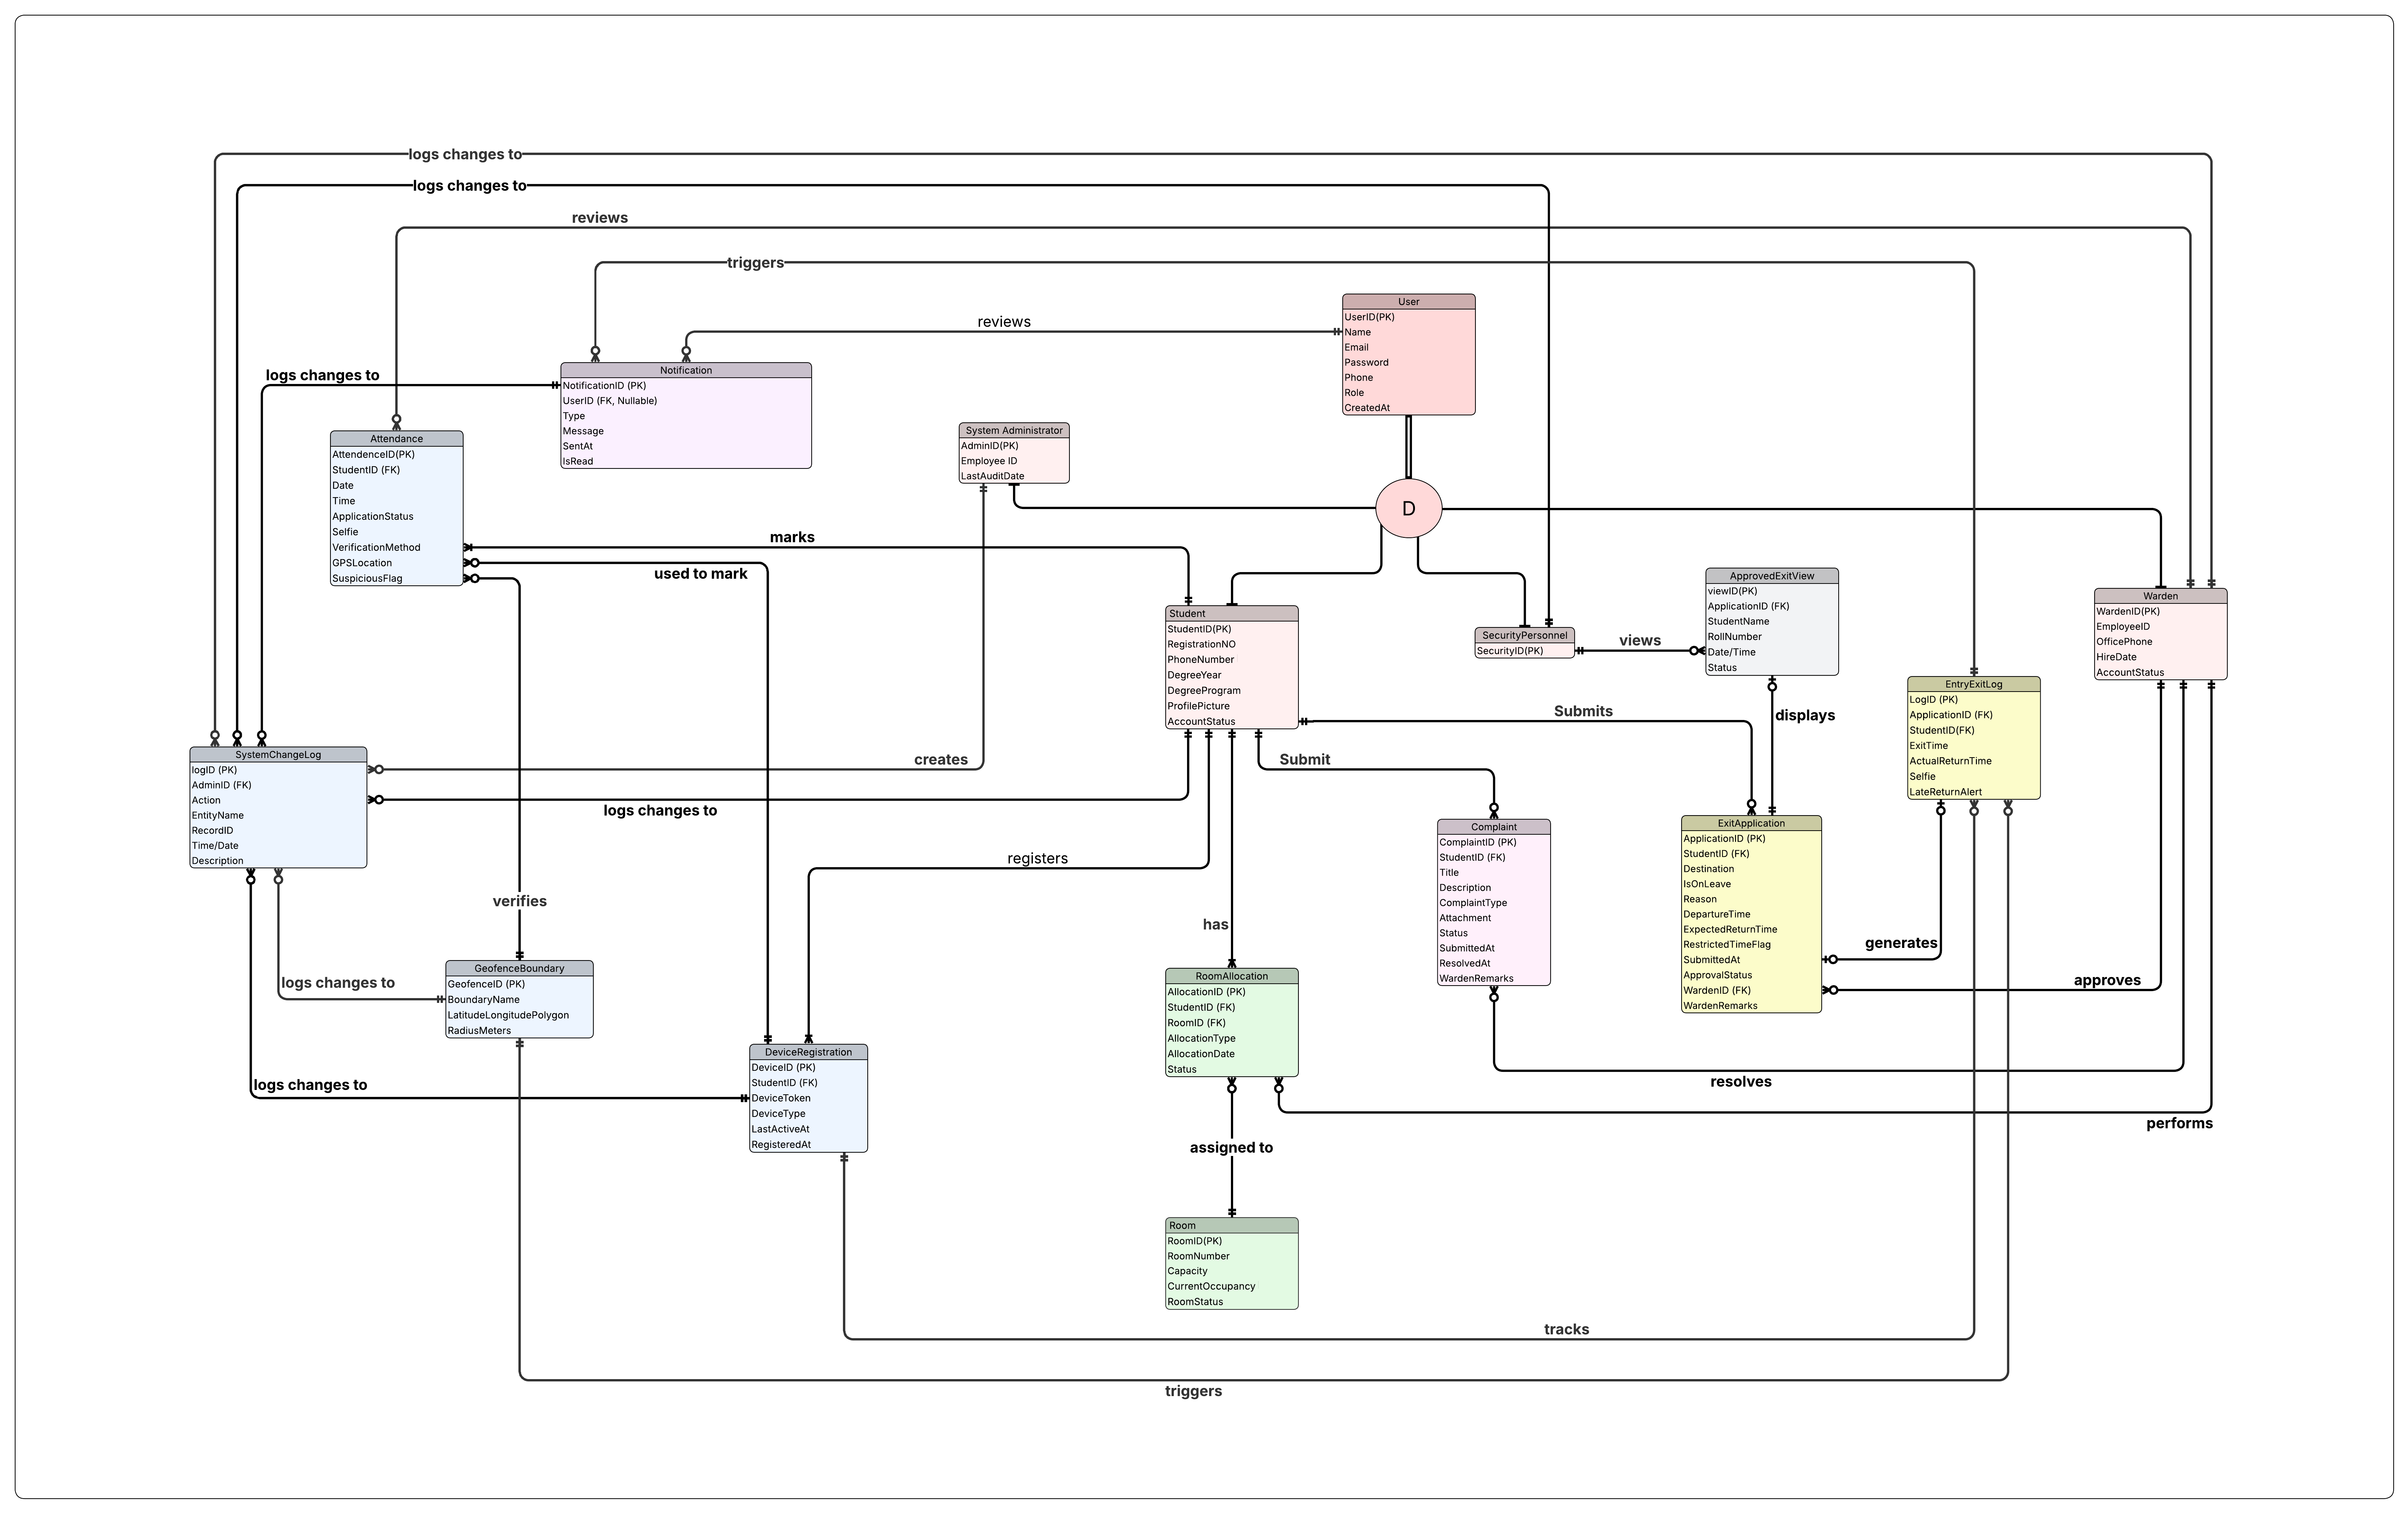
\includegraphics[width=0.9\textwidth]{SHMS_ERD.png}
    \caption{Entity Relationship Diagram of SHMS}
    \label{fig:erd}
\end{figure}

% ============================================================
\section{Advantages of the Proposed System}

\begin{itemize}
    \item Reduces paperwork through digital records
    \item Improves hostel security with geofence-based verification
    \item Provides centralized data management with full audit trail
    \item Improves communication efficiency via automated notifications
    \item Enables quick attendance and exit report generation
    \item Reduces human errors in attendance marking
    \item Provides efficient complaint handling with status tracking
    \item Enables fast application approval process for restricted-time exits
    \item Maintains organized room allocation 
    \item Prevents proxy attendance through temporary selfie capture
\end{itemize}

% ============================================================

\section{Conclusion}

The Smart Hostel Management System provides an efficient, secure, and centralized solution for hostel management operations. The system automates attendance management (with geofence + selfie), room allocation with full history tracking, complaint handling, entry/exit monitoring, and application approval management. The proposed database design uses a supertype-subtype structure (User with four subtypes) and includes 15 fully normalized entities. The SystemChangeLog entity ensures complete audit trail for all admin actions. The Entity Relationship Diagram developed in this milestone provides a strong foundation for implementation of the Smart Hostel Management System.

% ============================================================
\section{Teamwork \& Professional Conduct}

\begin{itemize}
   
    \item Regular coordination meetings were held
    \item Each member actively contributed and reviewed the final deliverables
    \item All sources (draw.io, Lucidchart) and AI assistance are disclosed in the AI appendix
\end{itemize}

% ============================================================
\section{AI Prompts Appendix}

The following AI prompts were used during project analysis and report preparation:

\begin{enumerate}
    \item Identify entities and attributes for hostel management system with geofence and temporary selfie 
    \item Generate business rules for attendance deadline, leave handling, and late return alerts
    \item Create Crow's Foot ERD relationships with proper cardinalities
\end{enumerate}

All technical decisions (entities, relationships, cardinalities, business rules) were made by the team after analysis. AI was used only for help or clearing the confusions, LaTeX formatting, and validation of design consistency.

% ============================================================
\section*{GitHub Repository}

The complete project source code, database schema, and ERD files are available on GitHub at the following link:

\vspace{0.5cm}

\centering
\href{https://github.com/Muhammad-Ahmad-99/Smart-Hostel-Management-System.git}{\fbox{\parbox{0.8\textwidth}{\centering \Large\bfseries https://github.com/Muhammad-Ahmad-99/Smart-Hostel-Management-System.git}}}

\vspace{0.5cm}

The repository contains:
\begin{itemize}
    \item Complete SQL database schema
    \item ERD diagrams (JPEG format)
    \item Project documentation
\end{itemize}

\end{document}
\end{document}